% Chapter 2: Background and Related Work
\chapter{Background and Related Work}
\label{chap:background}

% WHY: Establishing context and significance
% This section situates the thesis within the broader research landscape, clarifying why the problem matters and how the work advances the field.

\section{Historical Context and Evolution}

% Explain the origins and evolution of LLMs and ontologies in education, without repeating the introduction.
The intersection of artificial intelligence and education has evolved rapidly, with Large Language Models (LLMs) and ontological knowledge representation emerging as transformative technologies. Early educational technologies focused on rule-based systems and static content delivery. The advancement of LLMs enabled dynamic, context-aware interactions, while ontologies brought structured, machine-interpretable knowledge to educational platforms \cite{funk2023neuro}.

% Real-life analogy: Think of LLMs as talented tutors who can answer any question, and ontologies as the curriculum guide ensuring the tutor stays on track.

\section{Significance and Motivation}

% WHY: Why is this research important now?
Despite LLMs' promise, their tendency to hallucinate that is to generate plausible but incorrect information, poses a critical barrier in high-stakes domains like STEM education \cite{zhang2024survey, ji2023survey}. Ontologies offer a way to constrain and verify LLM outputs, but integrating these approaches remains an open challenge. Addressing this gap is essential for building trustworthy, adaptive educational systems.

% Key takeaway: The reliability of AI in education hinges on bridging the gap between flexible language models and structured domain knowledge.

\section{Review of Existing Literature}

% WHAT: What has been done before? How does it relate to your work?
\subsection{LLMs in Education}
Recent studies highlight LLMs' ability to personalize learning, generate content, and provide instant feedback. However, their lack of domain knowledge leads to factual errors, especially in technical subjects \cite{huang2024survey, su2024confabulation}.

\subsection{Ontologies in Educational Technology}
Ontologies have been used to structure curricula, model learner knowledge, and support adaptive learning paths \cite{liu2024ontology, wiley2024stem}. They enable explicit representation of concepts and relationships, supporting automated reasoning and assessment.

\subsection{Hybrid and Knowledge-Enhanced Systems}
Emerging research explores combining LLMs with ontologies or knowledge graphs to improve accuracy and reasoning \cite{hartl2024knowledge, funk2023neuro, arxiv2024ontology}. These hybrid systems show promise in reducing hallucinations and supporting context-aware responses, but practical, scalable solutions for real-time educational use are still lacking.

% Funnel structure: Start broad (AI in education), then focus on LLMs, ontologies, and finally their integration.

\section{Identified Gaps in Knowledge}

% WHAT: What is missing in the literature?
While prior work demonstrates the potential of both LLMs and ontologies, few studies have achieved seamless, real-time integration for STEM education. Key gaps include:
\begin{itemize}
    \item Lack of scalable frameworks for ontology-driven LLM verification in educational settings
    \item Limited empirical evaluation of hallucination mitigation in real-world classrooms
    \item Insufficient personalization and adaptability in existing hybrid systems
\end{itemize}

% Real-life analogy: Existing systems are like having a knowledgeable teacher and a strict curriculum, but no way for them to communicate in real time.

\section{Necessity, Relevance, and Innovation of This Study}

% WHY: Why is your work needed and how is it new?
This thesis addresses these gaps by proposing a novel framework that tightly integrates ontological knowledge with LLM reasoning for STEM education. The approach enables:
\begin{itemize}
    \item Real-time, ontology-based verification of LLM outputs
    \item Adaptive, context-aware tutoring tailored to individual learners
    \item Systematic reduction of hallucinations without sacrificing interactivity
\end{itemize}
By advancing the state of the art, this work lays the foundation for reliable, scalable, and effective AI-driven education.

% Key takeaway: The research is necessary to ensure AI can be trusted in education, and innovative in its real-time, ontology-driven approach.

% End with a transition to the next chapter
This background and literature review establish the foundation for the methodology presented in the following chapter.

\section{Large Language Models in Education}

\subsection{Evolution and Capabilities}
Large Language Models represent a significant advancement in artificial intelligence, particularly in natural language processing and understanding \cite{ji2023survey}. These models, trained on vast amounts of text data, have demonstrated remarkable capabilities in:

\begin{itemize}
    \item Natural language understanding and generation
    \item Context-aware responses and explanations
    \item Adaptation to various domains and topics
    \item Multi-turn conversations and reasoning
\end{itemize}

Recent developments in hybrid alignment training \cite{wang2024hybrid} and search engine augmentation \cite{vu2024freshllms} have further enhanced these capabilities.

% --- BEGIN: LLM Timeline TikZ Diagram ---
% This TikZ diagram visually summarizes the historical evolution of Large Language Models (LLMs) in education.
% Each milestone is marked on a horizontal timeline, with dates and brief descriptions.
% To modify or add milestones, simply update the 'milestones' list below.
% Requires: \usepackage{tikz} in the preamble.
\begin{figure}[ht]
    \centering
    % Timeline diagram using TikZ
    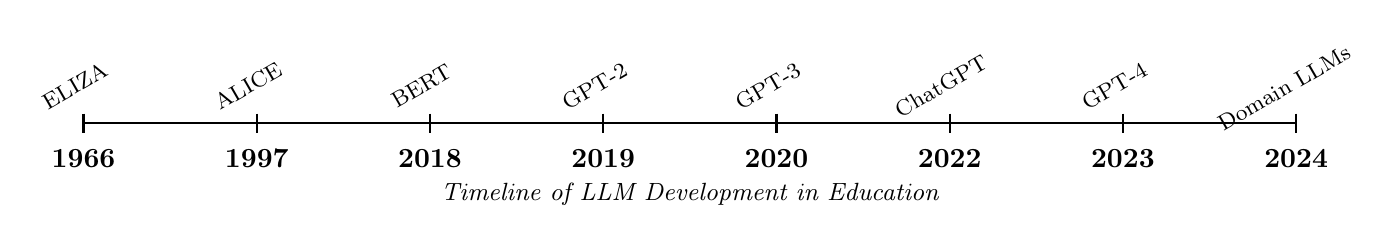
\begin{tikzpicture}[xscale=2.2, yscale=1.2]
        % --- Timeline axis ---
        \draw[thick] (0,0) -- (7,0);
        % --- Milestones: (year, label, description) ---
        % List of milestones (edit here to add/remove events)
        \foreach \x/\year/\label in {
            0/1966/ELIZA, % First chatbot
            1/1997/ALICE, % Pattern-matching chatbot
            2/2018/BERT, % Contextual embeddings
            3/2019/GPT-2, % Large-scale LLM
            4/2020/GPT-3, % Few-shot learning
            5/2022/ChatGPT, % Conversational LLM
            6/2023/GPT-4, % Multimodal, advanced reasoning
            7/2024/Domain LLMs % MedPaLM, MathGPT, etc.
        } {
            % Draw milestone tick
            \draw[thick] (\x,0.1) -- (\x,-0.1);
            % Year label
            \node[align=center, font=\bfseries, below=6pt] at (\x,0) {\year};
            % Event label
            \node[align=center, font=\footnotesize, above=8pt, rotate=30] at (\x,0) {\label};
        }
        % --- Axis label ---
        \node[below=18pt, font=\small\itshape] at (3.5,0) {Timeline of LLM Development in Education};
    \end{tikzpicture}
    \caption{Timeline of LLM Development in Education. Key milestones are shown from the first chatbot (ELIZA) to modern, domain-specific LLMs. This visual contextualizes the rapid evolution and growing impact of LLMs in educational technology.}
    \label{fig:llm-timeline}
\end{figure}
% --- END: LLM Timeline TikZ Diagram ---

% Figure 2.1: Timeline of LLM Development in Education

\subsection{Limitations and Challenges}
Despite their capabilities, LLMs face several critical challenges in educational applications \cite{zhang2024survey}:

\begin{itemize}
    \item \textbf{Hallucination:} Generation of plausible but incorrect information
    \item \textbf{Contextual Understanding:} Limited ability to maintain consistent context
    \item \textbf{Domain Specificity:} Challenges in specialized STEM topics
    \item \textbf{Verification:} Difficulty in validating generated responses
\end{itemize}

Recent research has shown that hallucinations can be both a limitation and a potential source of creative problem-solving \cite{su2024confabulation}. However, in educational contexts, particularly in STEM fields, accuracy remains paramount \cite{zuo2025medhallbench}.

% --- BEGIN: Taxonomy of LLM Hallucinations TikZ Diagram ---
% This TikZ diagram presents a taxonomy of hallucinations produced by LLMs in educational contexts.
% The root node is "LLM Hallucinations in Education", branching into four main types:
%   - Factual, Logical, Contextual, and Pedagogical Hallucinations.
% Each branch includes a brief description or example for clarity.
% To modify or add categories, update the tree structure below.
% Requires: \usepackage{tikz} in the preamble.
\begin{figure}[ht]
    \centering
    % Taxonomy tree diagram using TikZ
    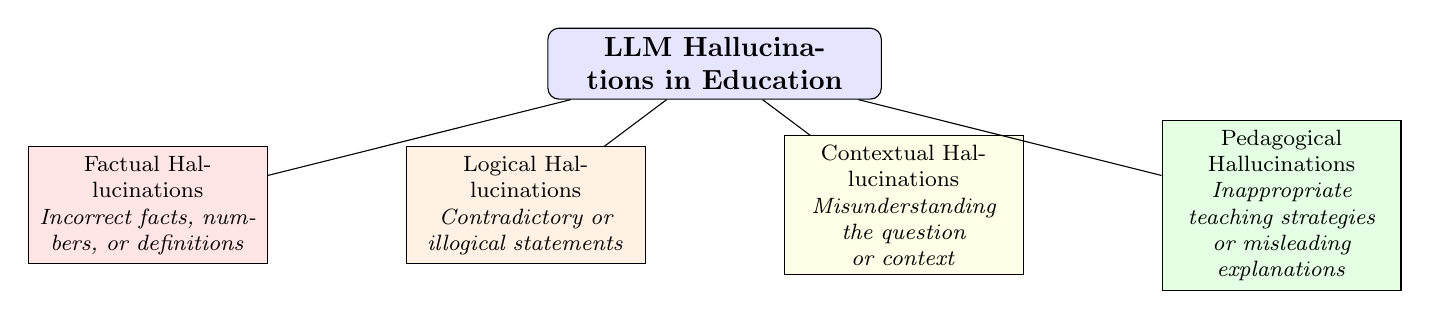
\begin{tikzpicture}[
        level 1/.style={sibling distance=48mm, level distance=18mm},
        level 2/.style={sibling distance=24mm, level distance=18mm},
        every node/.style={font=\footnotesize, align=center}
    ]
        % Root node
        \node[draw, rounded corners, fill=blue!10, font=\bfseries, text width=40mm, align=center] {LLM Hallucinations in Education}
            % First level branches
            child {node[draw, fill=red!10, text width=28mm] {Factual Hallucinations\\\textit{Incorrect facts, numbers, or definitions}}}
            child {node[draw, fill=orange!10, text width=28mm] {Logical Hallucinations\\\textit{Contradictory or illogical statements}}}
            child {node[draw, fill=yellow!10, text width=28mm] {Contextual Hallucinations\\\textit{Misunderstanding the question or context}}}
            child {node[draw, fill=green!10, text width=28mm] {Pedagogical Hallucinations\\\textit{Inappropriate teaching strategies or misleading explanations}}};
    \end{tikzpicture}
    \caption{Taxonomy of LLM Hallucinations in Education. The diagram categorizes common types of hallucinations produced by language models in educational settings, clarifying the risks and motivating the need for ontology-based verification.}
    \label{fig:llm-hallucination-taxonomy}
\end{figure}
% --- END: Taxonomy of LLM Hallucinations TikZ Diagram ---

\section{Ontologies in Knowledge Representation}

\subsection{Fundamentals of Ontological Engineering}
Ontologies provide a formal, structured representation of knowledge within a domain \cite{nananukul2023halo}. Key components include:

\begin{itemize}
    \item \textbf{Classes and Hierarchies:} Representing concepts and their relationships
    \item \textbf{Properties:} Defining characteristics and relationships
    \item \textbf{Instances:} Specific examples within the ontology
    \item \textbf{Axioms:} Rules and constraints governing relationships
\end{itemize}

% --- BEGIN: Example Ontology Structure Figure ---
% This figure illustrates a simplified ontology for mathematical functions, adapted from Hare & Tang (2024).
% The ontology shows how the broad concept of "Function" branches into sub-concepts (e.g., Linear, Quadratic),
% exemplifying how ontologies structure domain knowledge for AI-driven education.
% The image is stored in src/figures/diagrams/ExampleOntology.png for modular project organization.
% Reference: Hare, R. & Tang, Y. (2024). Ontology-driven Reinforcement Learning for Personalized Student Support. arXiv:2407.10332.
\begin{figure}[ht]
    \centering
    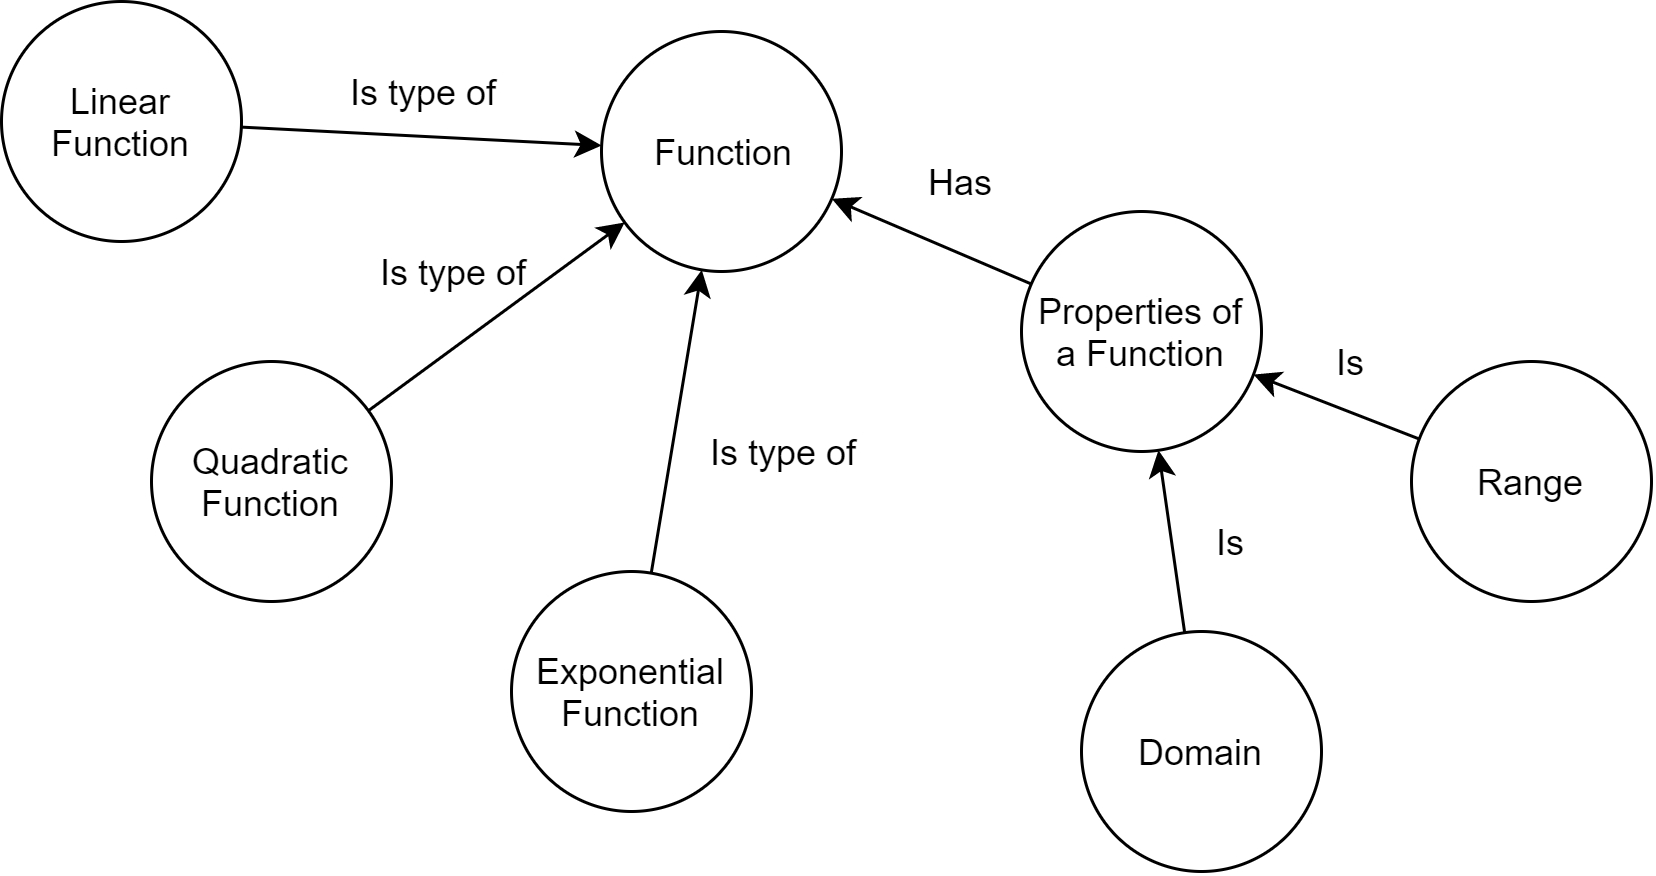
\includegraphics[width=0.8\textwidth]{figures/diagrams/ExampleOntology.png}
    \caption{Sample ontology structure for STEM education, focusing on mathematical functions and their sub-concepts. Adapted from \cite{hare2024ontology}. This diagram demonstrates how ontologies can organize and relate key concepts, supporting adaptive and personalized learning in AI-driven educational systems.}
    \label{fig:ontology-math-functions}
\end{figure}
% --- END: Example Ontology Structure Figure ---

\section{Key Concepts and Definitions}

\subsection{Core Terminology}
This section defines key terms used throughout this thesis:

\begin{itemize}
    \item \textbf{Ontology:} A structured framework representing knowledge within a specific domain, defining concepts, properties, and relationships for clear communication and effective information retrieval in human-AI interaction.
    
    \item \textbf{Knowledge Model:} A structured representation of information that explicitly defines concepts, relationships, and logic within a particular domain, facilitating consistent interpretation and accurate reasoning.
    
    \item \textbf{Large Language Model (LLM):} An advanced AI model trained on extensive textual data, capable of generating human-like text, understanding context, and performing complex reasoning tasks.
    
    \item \textbf{Virtual Environment:} Digitally simulated spaces designed to mimic real-world scenarios, supporting user immersion and interaction through various sensory elements.
    
    \item \textbf{Digital Avatars:} Virtual representations of users or characters within digital environments, embodying human-like traits to enhance interaction quality.
    
    \item \textbf{Ontology-driven Integration:} The process of using structured ontologies to unify different data sources or systems, ensuring coherent communication and consistency across applications.
    
    \item \textbf{AI-Human Interaction:} The exchange of information between AI systems and human users, relying on clear understanding and context-aware responses.
    
    \item \textbf{Semantic Knowledge:} Contextually interpreted information that enables systems to understand implied meanings and relationships between concepts.
    
    \item \textbf{Knowledge Graph:} A structured data representation organizing information into interconnected nodes and edges, enabling effective visualization and interpretation of complex relationships.
\end{itemize}

